\section{Muon chambers}
\label{fig1:cms_muon2}
%Fig\pdfcomment[author={FIG COURTESY}]{http://cms.web.cern.ch/news/muon-drift-tubes}}
Detection of muons was the primary physics motive for the CMS experiment. Being
a minimum ionizing particle, the muon traverses most part of CMS without
losing much energy in the calorimeters. Except for the muons, other particles
produced in the collision are stopped either in ECAL or HCAL. In view of this,
muon chambers are placed at the outermost side of CMS where only muons are
supposed to be detected. The muon chambers have a different configuration in the
barrel and endcap regions. When a muon passes through the muon chambers, filled
with gases, atomic electrons are knocked out. Subsequently, the current corresponding
to these electrons is amplified and stored. As shown in Figure~\ref{fig:cms_mu},
the CMS experiment has the following three types of the muon chambers: drift tubes (DTs),
cathode strip chambers (CSCs), and resistive plate chambers (RPCs). The momentum resolution of 
the muon detector is 10\% (20\%) in the barrel (endcap) region for a muon with 
\pt = 40 \GeV. Various properties and parameters of the muon subsystem are listed in 
Table~\ref{tab:muChamberParam}. A brief description of these subsystems is given below.
\begin{figure}
\centering
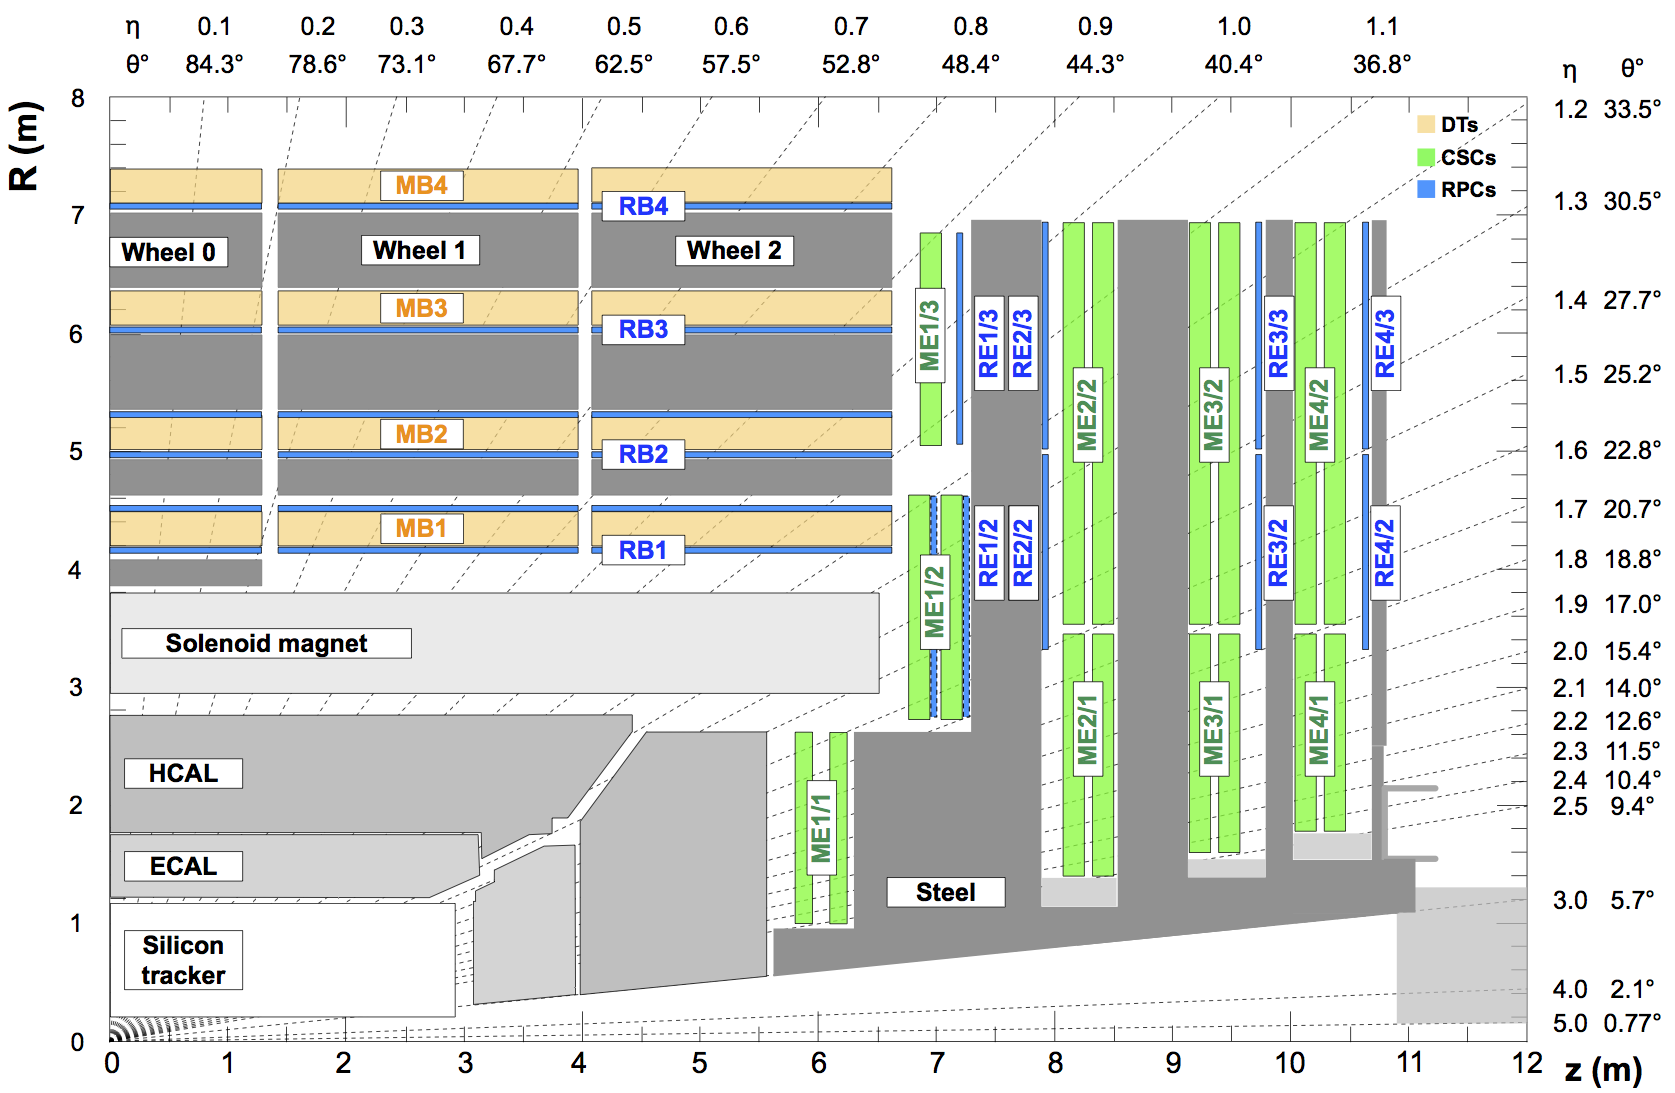
\includegraphics[width=0.75\linewidth]{Experiment/CMS/Image/mu2.png}
\caption{Location of the various sub-detectors of the CMS 
	\cite{Sirunyan:2018fpa}. The DTs and CSCs are placed in barrel and 
	endcap regions. The RPCs are placed in both regions. The muon chamber
	in the barrel region is formed by placing three \dq{wheels} side-by-side
	along the $z$-axis whereas in the endcap regions different segments
	of RPC and CSC are placed along the radial direction.}
\label{fig:cms_mu}
\end{figure}
\begin{table}
   \caption{Various properties and parameters of the CMS muon subsystems 
	\cite{Sirunyan:2018fpa}.}
   \centering
   \begin{tabular}{cccc}
     \hline
     \hline
     Muon subsystem                &    DT                               &    CSC                  & RPC              \\
     \hline
     \hline
     $|\eta|$ coverage         & 0.0--1.2                            & 0.9--2.4                & 0.0--1.9         \\
     Number of stations            & 4                                   & 4                       & 4                \\
     Number of chambers            & 250                                 & 540                     & Barrel: 480      \\
                                   &                                     &                         & Endcap: 576      \\
     Number of layers per chamber      & \textit{R}-$\phi$: 8; \textit{z}: 4 & 6                       & 2 in RB1 and RB2 \\
                                   &                                     &                         & 1 elsewhere      \\
     Number of readout channels    & 172000                             & Strips: 266112         & Barrel: 68136   \\
                                   &                                     & Anode channels: 210 816 & Endcap: 55296   \\
     Percentage of active channels &   98.4\%                            &   99.0\%                &  98.3\%          \\
     \hline
   \end{tabular}
   \label{tab:muChamberParam}
 \end{table}

\begin{itemize}[leftmargin=*]
\item \textbf{Drift tube}: The DTs are placed in the barrel region. 
A schematic diagram of a DT is shown in Figure~\ref{fig:cms_dt}, where the 
red dots are the aluminum wires pointing into the page. The region between the wires 
are filled 85\% with Argon (Ar) and 15\% with $\rm{CO}_2$ gases. When a muon passes through 
the DTs, atomic electrons are knocked-out of the gases. The anode wires attract electrons
towards themselves. The distance traveled by electrons up to the anode wire is shown
by horizontal arrows. The information about the length of such arrows gives direction
in which the muon could have traversed inside the DTs, which give the $z$ and $\phi$ 
coordinates of the muon.
\begin{figure}
\centering
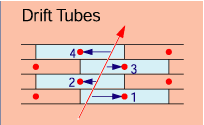
\includegraphics[width=0.50\linewidth]{Experiment/CMS/Image/DT.png}
\caption{Schematic view of one of the DTs of the muon chamber \cite{Collaboration_2008_CMS}. 
	The red dots are the aluminum wires pointing into the page, the red arrow is the
	direction of an incoming muon, and the horizontal blue lines are the 
	distance traveled by secondary electrons.}
\label{fig:cms_dt}
\end{figure}

\item \textbf{Cathode strip chamber}: A schematic diagram of the cathode strip
	chamber is shown in Figure~\ref{fig:cms_csc}. The CSC is placed in the
	endcap region where particle multiplicity is very high. It consists
	of anode wires of gold-plated tungsten and cathode strips made of copper. 
	The wires and strips are placed perpendicular to each other. A 
	mixture of different gases consisting of 50\% CO$_2$, 40\% Ar, and 10\% 
	CF$_4$ is filled between anode and cathode. When muon passes
	through the CSC, atomic electrons are knocked out of the gasses and attracted
	towards the anode wires. Whereas the ions are attracted towards the cathode
	strips. Therefore, two coordinates is determined from the CSC,
	unlike the DT where only one coordinate is determined. 
\begin{figure}
\centering
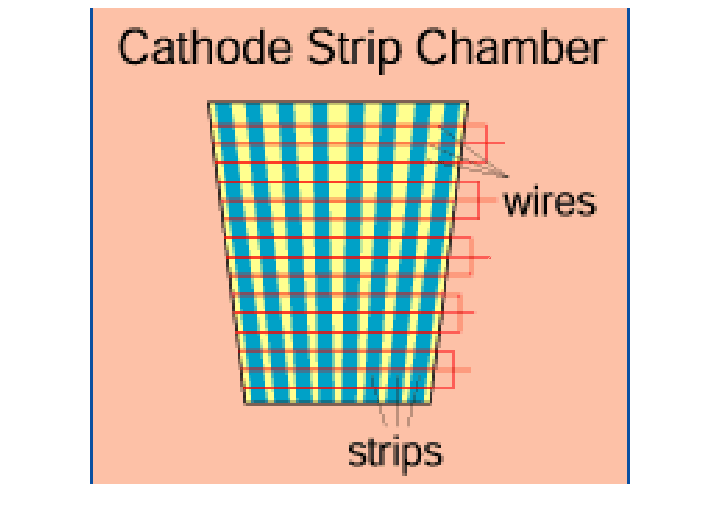
\includegraphics[width=0.50\linewidth]{Experiment/CMS/Image/CSC.png}
\caption{Schematic view of one of the cathode strip chambers~\cite{Collaboration_2008_CMS}. 
	The wires shown in red and cathode strips shown in cyan are placed perpendicular to each
	other.}
\label{fig:cms_csc}
\end{figure}

\item \textbf{Resistive plate chamber}: The response from the RPC is very
	fast, hence, it helps in quick triggering (see Section~\ref{ss:secTrig}).
	The time resolution of the RPC is 3\unit{ns}.
	A schematic diagram of one of the RPCs is shown in Figure~\ref{fig:cms_rpc}.
	There are two resistive plates: one acts as the anode and the other as the cathode.
	Only the anode plate is transparent to the secondary electrons.
	The region between the plates is filled with a mixture of gases (95.2\% 
	C$_2$H$_2$F$_4$, 4.5\% i-C$_4$H$_{10}$,	and 0.3\% SF$_6$). When a muon 
	passes through the gases, atomic electrons are knocked out. These electrons are 
	picked up by anode strips placed above the anode plate. The momentum of a 
	muon is measured from the hit pattern in the strips. The muon information is 
	conveyed to the global muon trigger (see Section~\ref{ss:secTrig}). 
\begin{figure}
\centering
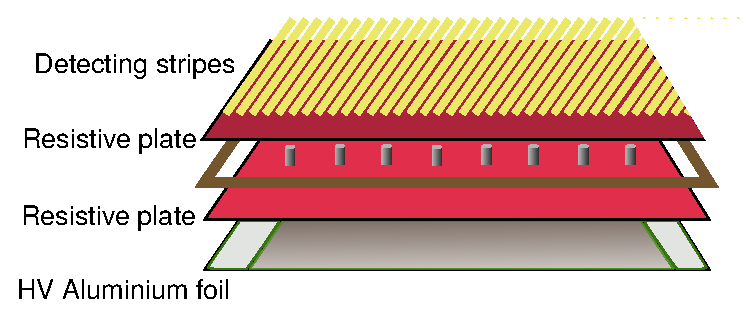
\includegraphics[width=0.65\linewidth]{Experiment/CMS/Image/RPC.pdf}
\caption{Schematic diagram of one of the RPCs. The cathode (bottom red plate) and 
	anode (top red plate) is separated by a separator (shown in gray). The
	region between the two plates is filled with gas. The anode is
	transparent to the secondary electrons. The orange strips (above anode)
	picks the secondary electrons. The high voltage aluminum foil is placed
	at the bottom. This figure is adopted from ~\cite{Collaboration_2008_CMS}.}
\label{fig:cms_rpc}
\end{figure}
\end{itemize}

